\documentclass[12pt]{article}
\usepackage[english]{babel}
\usepackage[utf8]{inputenc}
\usepackage{amsmath, amssymb, amsthm}
\usepackage{graphicx}
\usepackage{hyperref}
\usepackage[paperwidth=15.11in,paperheight=8.5in,margin=.75in]{geometry}
\usepackage{xcolor}
\usepackage{tikz}

\newcommand{\id}{\text{id}}
\newcommand{\od}{\text{od}}

\setlength{\topmargin}{0pt}
\setlength{\headsep}{0pt}
\textheight = 600pt

\title{Pruning Rules and Branching Heuristics for Edge Clique Cover}
\author{Ben Kallus}
\date{Wednesday, May 12, 2021}

\begin{document}
\maketitle

\begin{center} 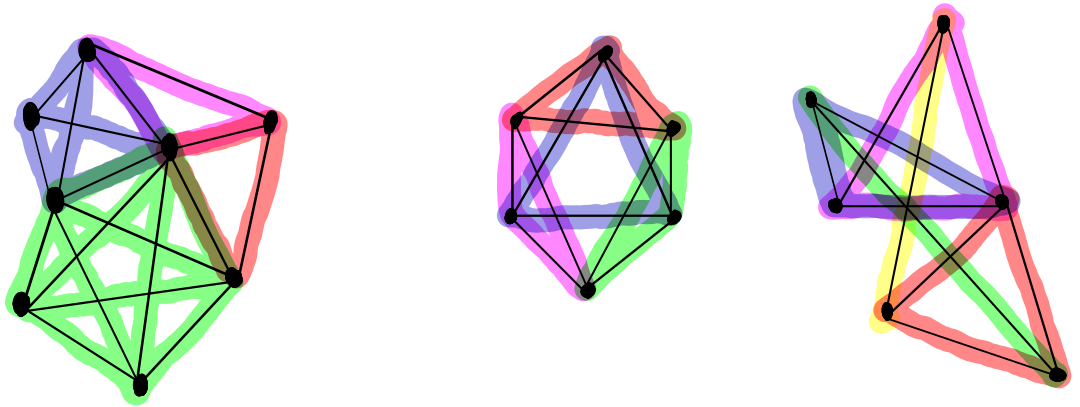
\includegraphics{fig1.png} \end{center}

\newpage
\section*{Graphs}
    %% A graph is a collection of vertices in which pairs of vertices may be connected with edges.
    \begin{center} 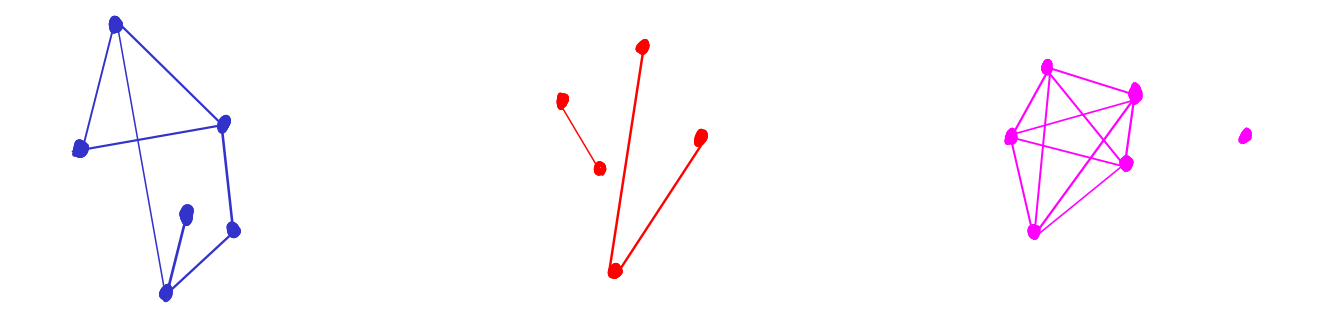
\includegraphics{fig0.png} \end{center}
    %% Graphs are useful for representing pairwise relationships between members of a set of objects. ie social networks, electrical grids, highway systems, 

\newpage
\section*{Complete Graphs}
    %% A complete graph is a graph in which every pair of distinct vertices is connected with an edge.
    \begin{center} 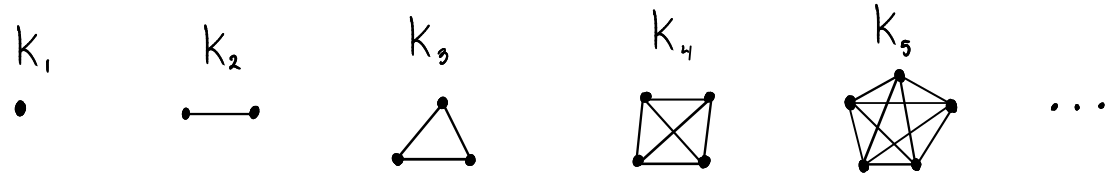
\includegraphics{fig5.png} \end{center}

\section*{Cliques}
    %% A clique in a graph G is a complete subgraph of G.
    %% So if G is a social network, a 5-clique in G represents a group of 5 people who all know each other.

    \begin{center} 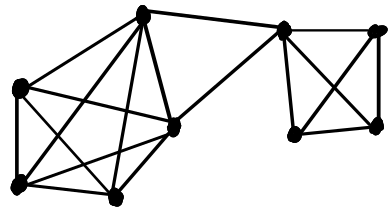
\includegraphics[scale=1.4]{fig13.png} \end{center}

\newpage
\section*{The Edge Clique Cover Problem}
    %% Given a graph, what is the smallest set of cliques I can find such that every edge in the graph is included in at least one clique?
    %% Be specific about edges, not just covering graph
    \begin{center}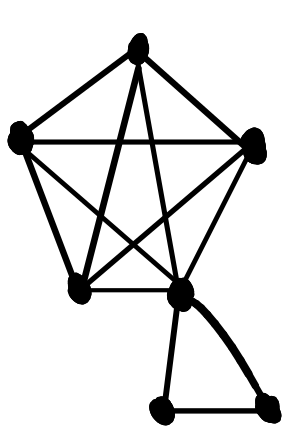
\includegraphics[scale=1]{fig11.png} \hspace{3in} 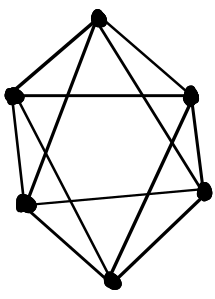
\includegraphics[scale=1.4]{fig12.png} \end{center}

    %% NP-Hard, APX-Hard

%\newpage
%\section*{Why it's Hard}

    %% Estimations
%    \begin{center} 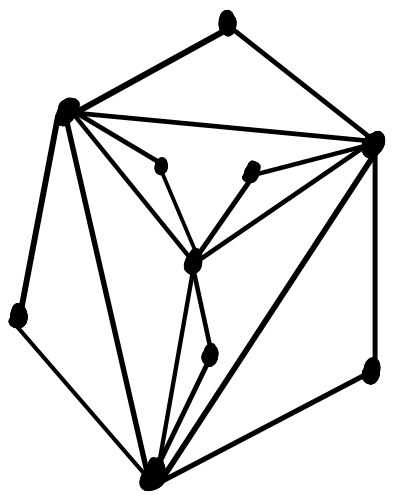
\includegraphics[scale=1.3]{fig14.png} \end{center}

\newpage
\section*{Reduction Rules}

    %% Gramm et al. 2008
    %% List reductions
    \begin{center} 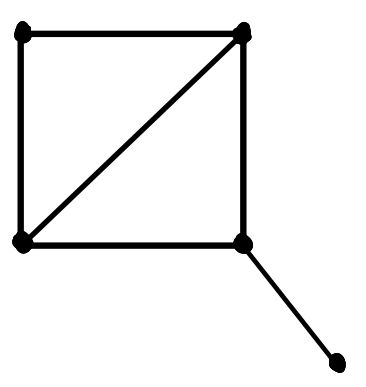
\includegraphics{fig15.png} \hspace{3in} 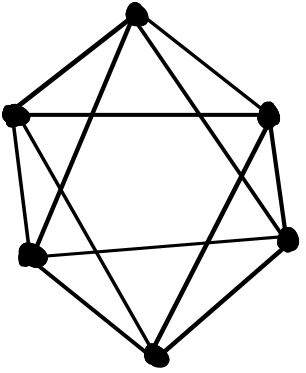
\includegraphics{fig17.png} \end{center}

\newpage
\section*{Branching}

    \begin{center} 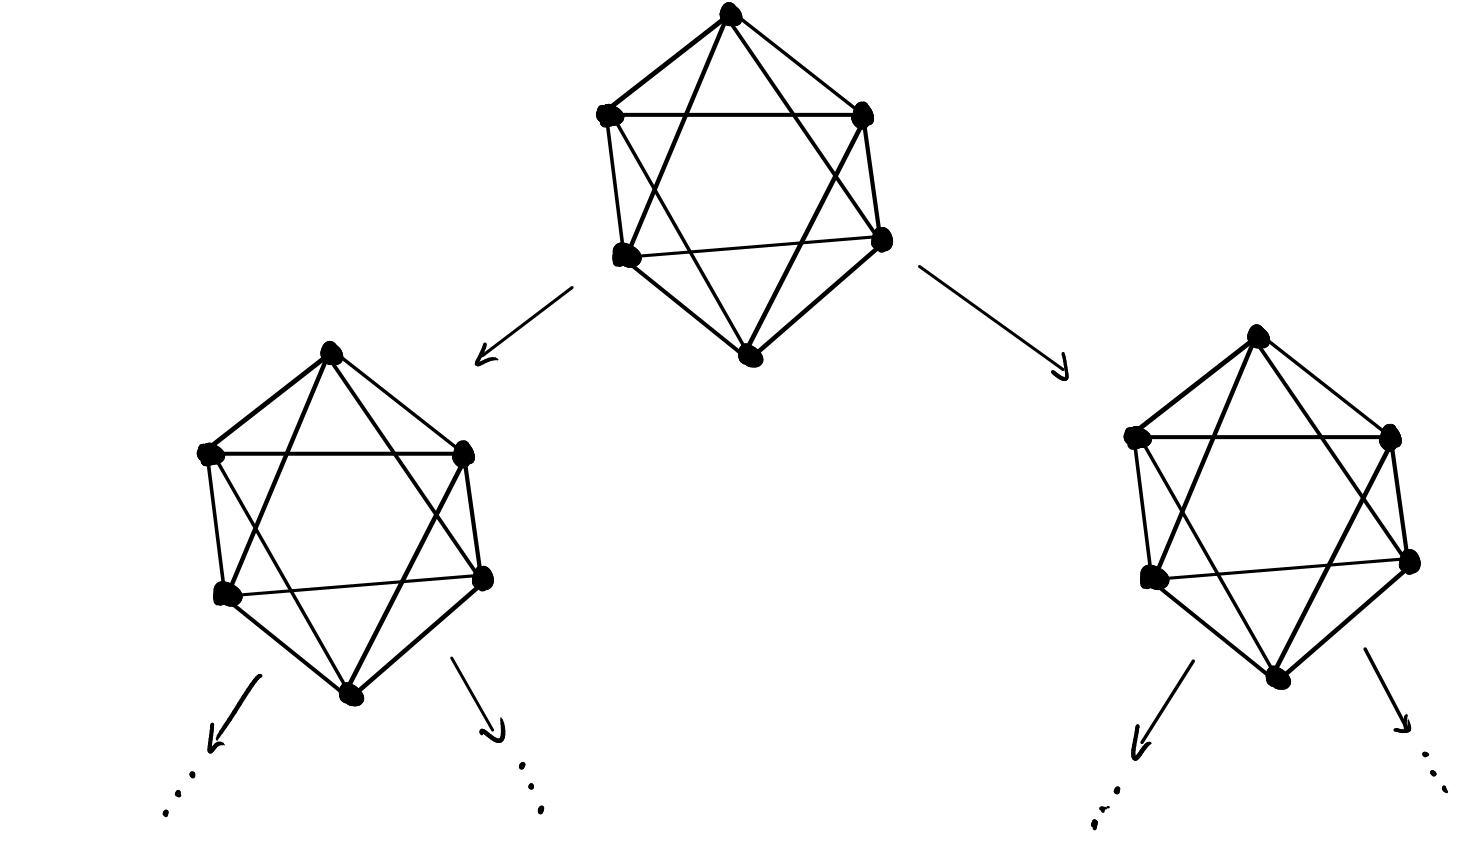
\includegraphics[scale=.75]{fig16.png} \end{center}

\newpage
\section*{Pruning}
    
    %% Mention that Gramm does no pruning at all.
    \begin{center} 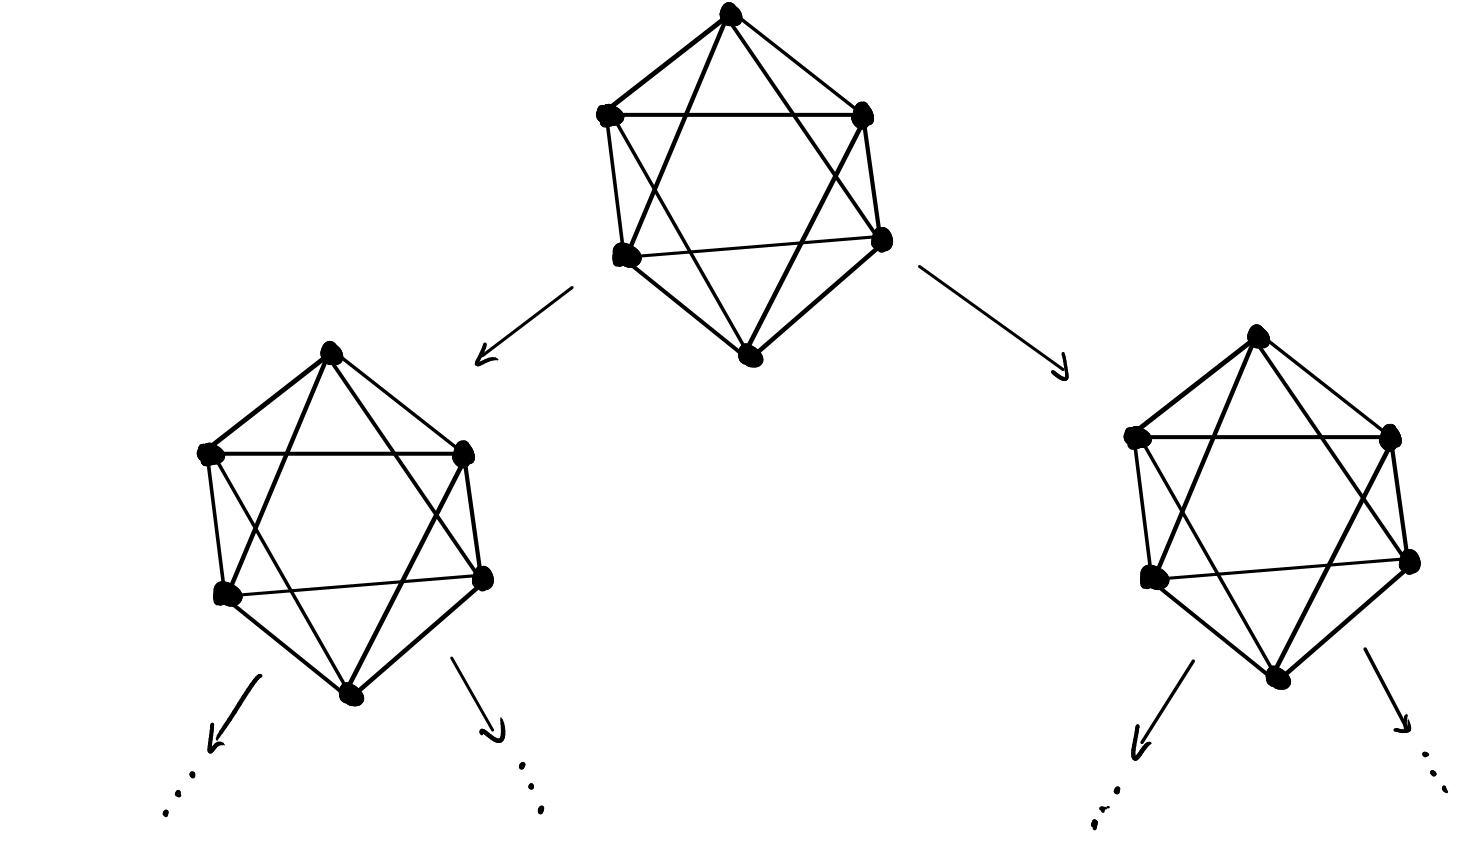
\includegraphics[scale=.75]{fig16.png} \end{center}

\newpage
\begin{center} No Pruning vs. Trivial Rule\\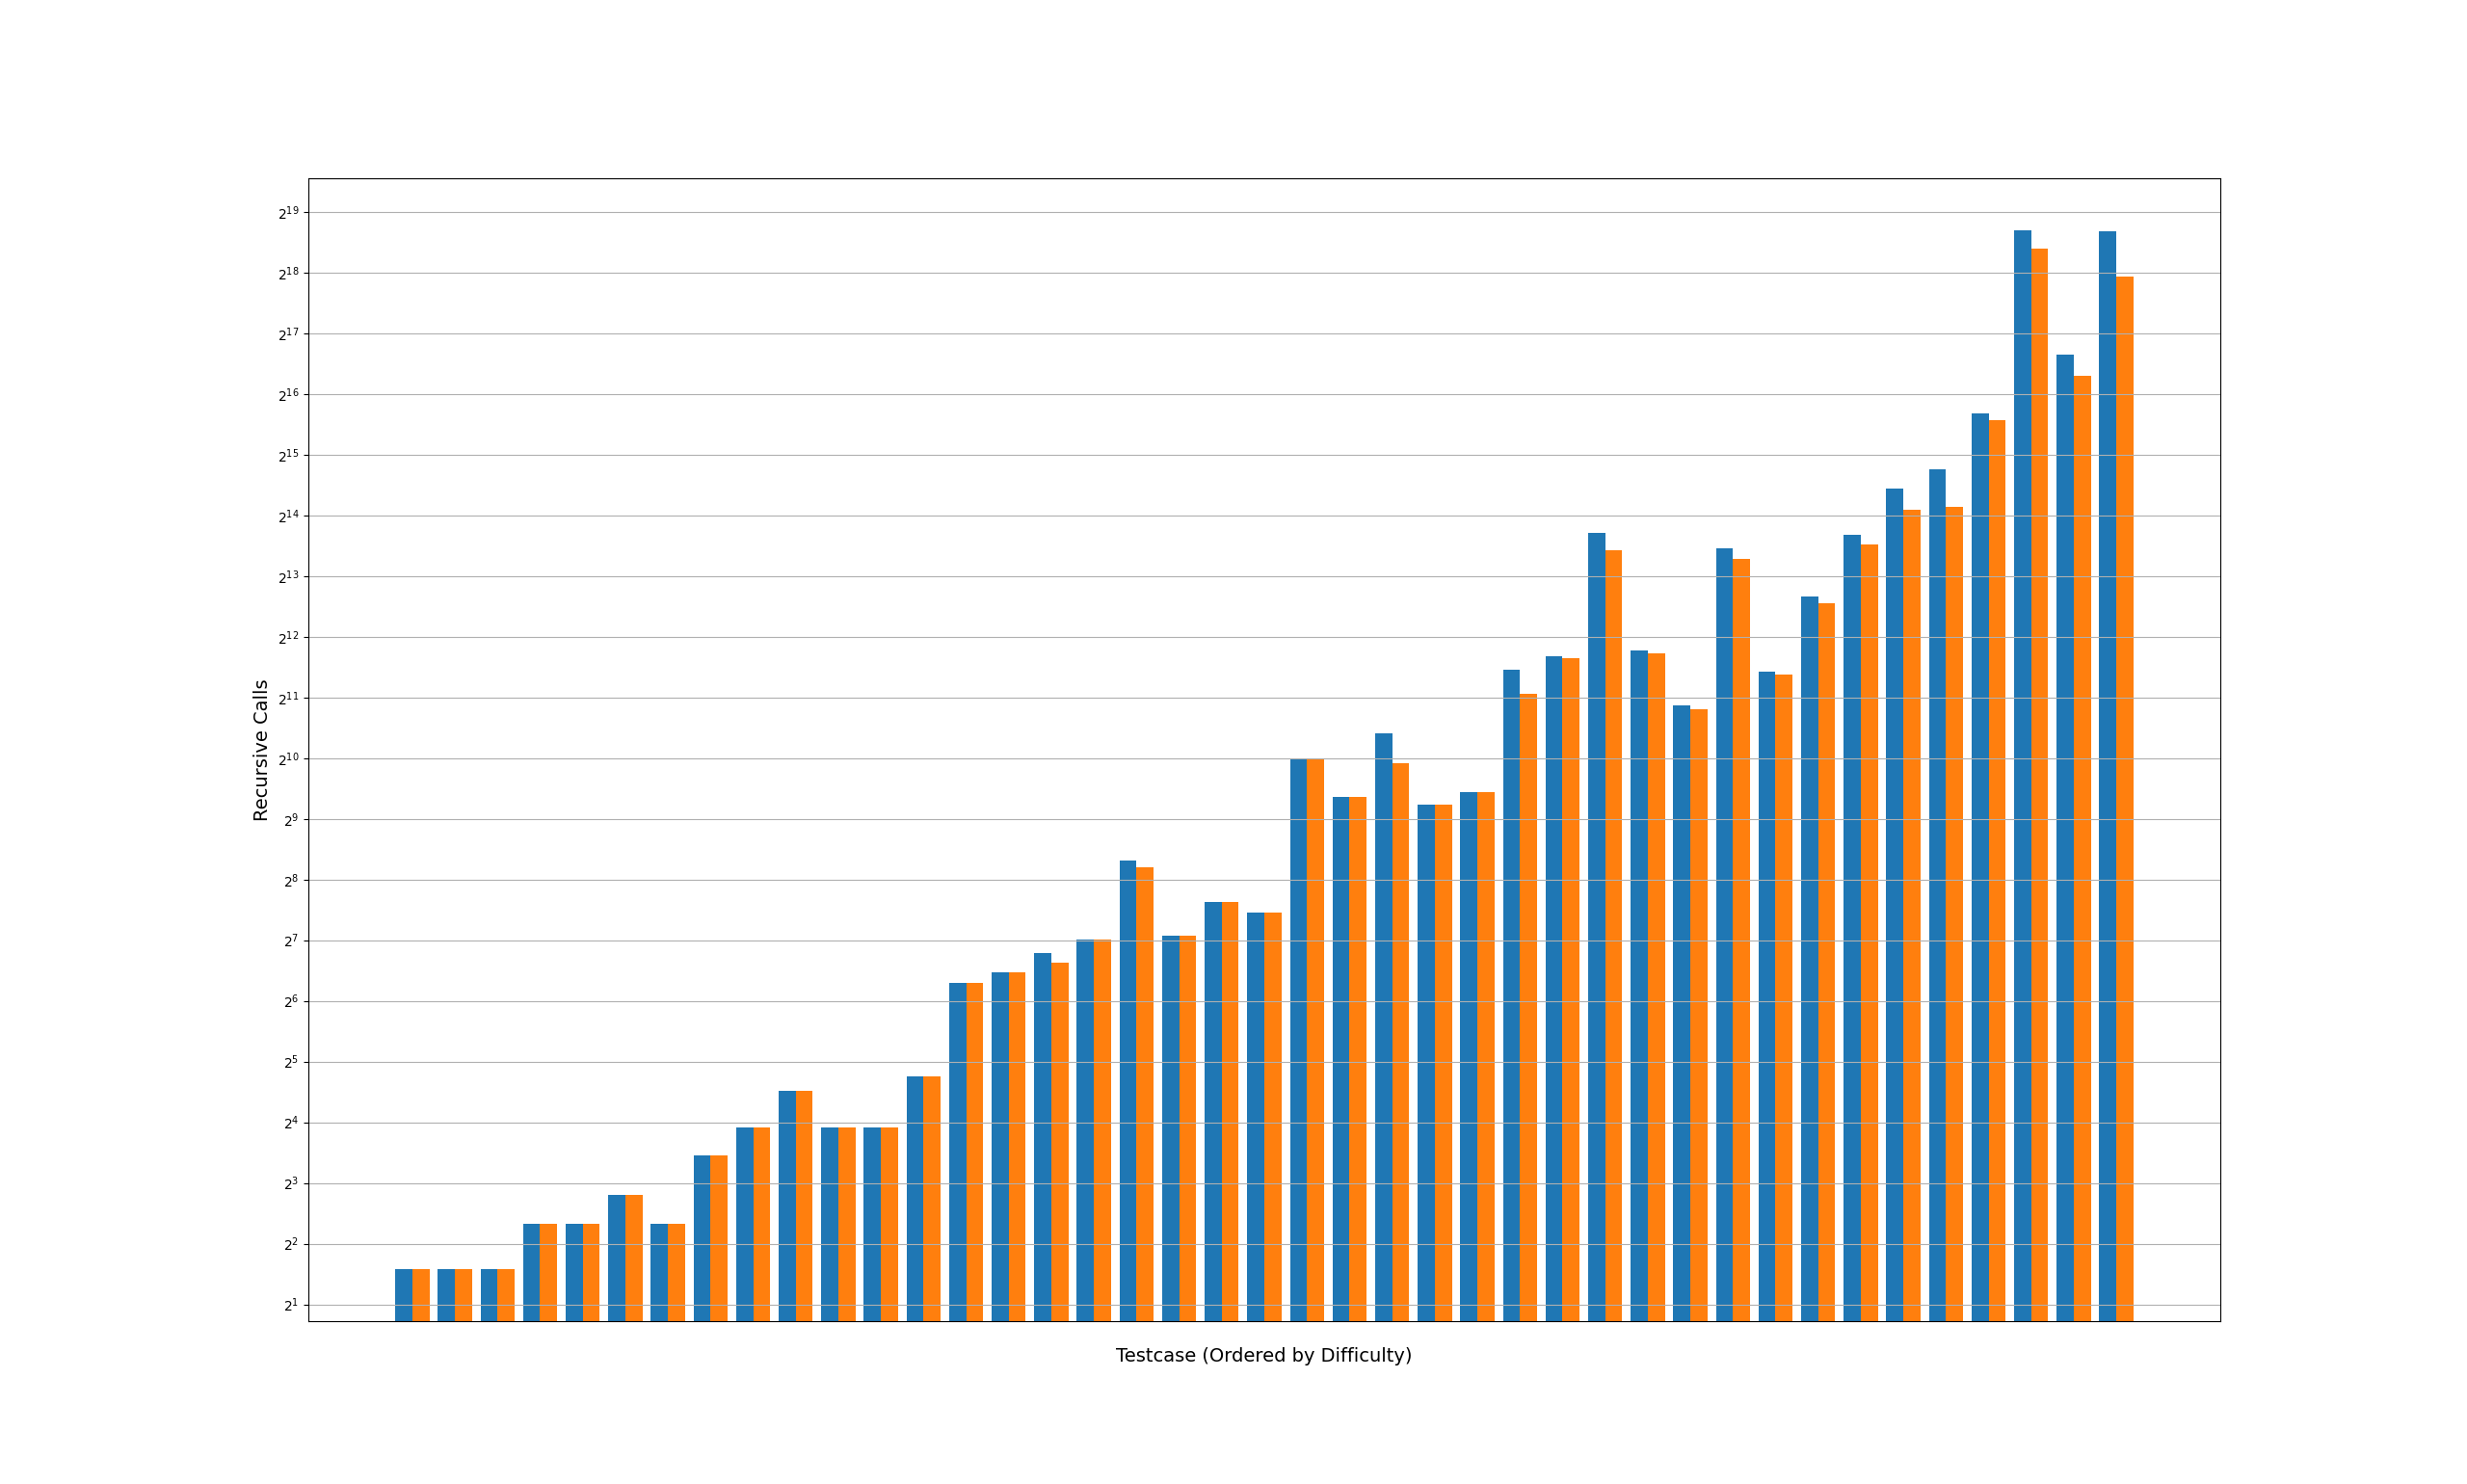
\includegraphics[scale=.5]{nonetrivial.png} \end{center}

\newpage
\section*{Pruning with Independent Sets}

    \hfill 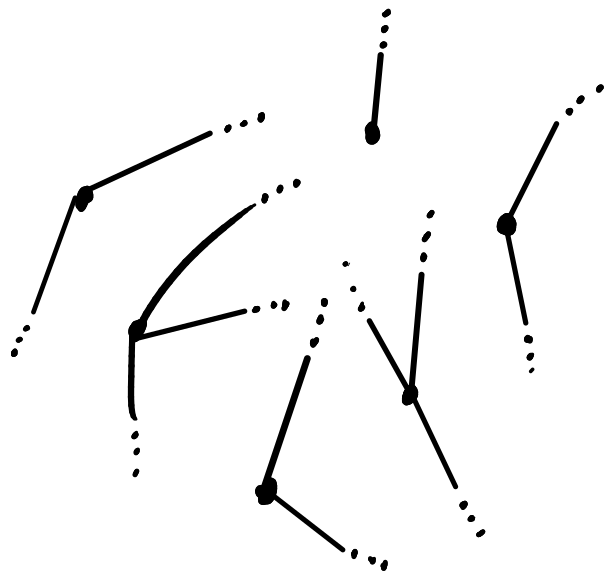
\includegraphics{fig18.png} \hspace*{\fill}

    %% Eliminate wasted effort in the search tree algorithm.
    %% Let's say we've found one cover of size 4.
    %% And we're halfway through finding another cover, and we've found 8 cliques so far.

\newpage
\begin{center} Trivial Rule vs. Vertex Rule\\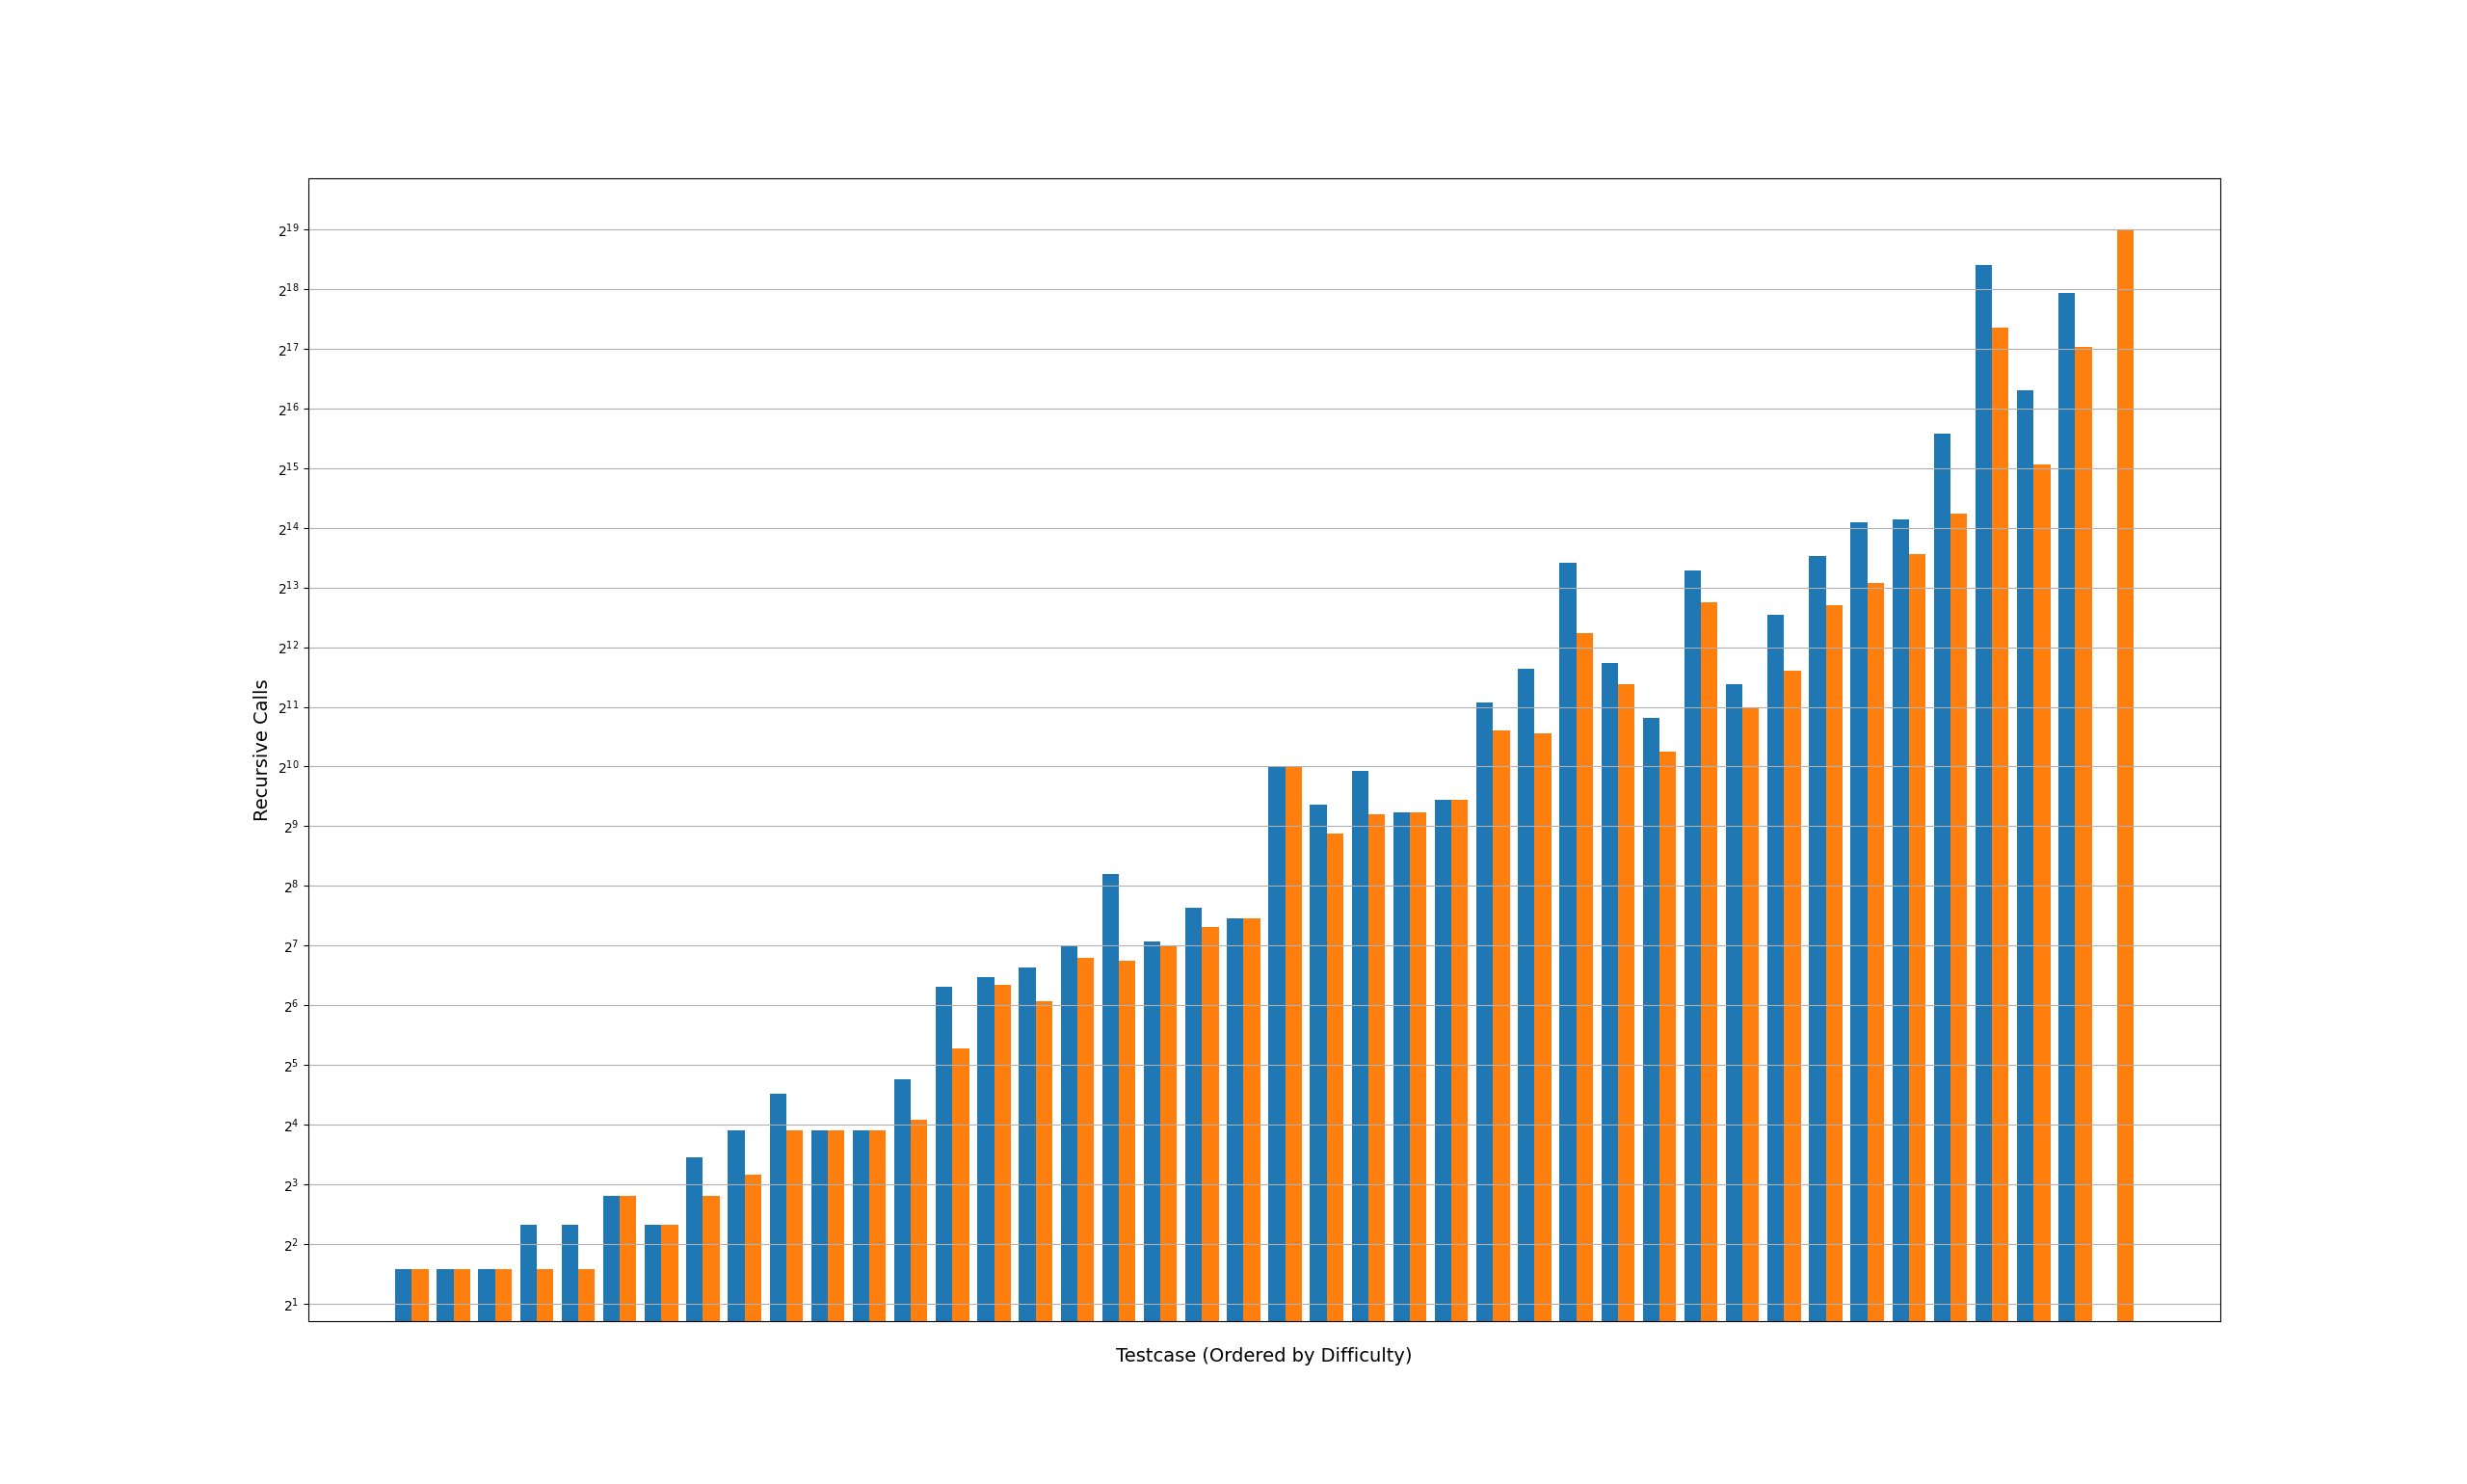
\includegraphics[scale=.5]{trivialvertex.png} \end{center}

\newpage
\section*{New Pruning Technique}

    \begin{center} 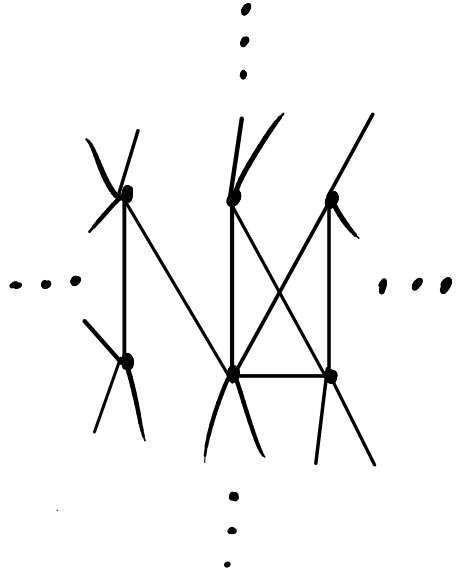
\includegraphics{fig19.png} \end{center}

    %% If we can build a big enough set, we can prune signficantly.

\newpage
\begin{center} Vertex Rule vs. Edge Rule\\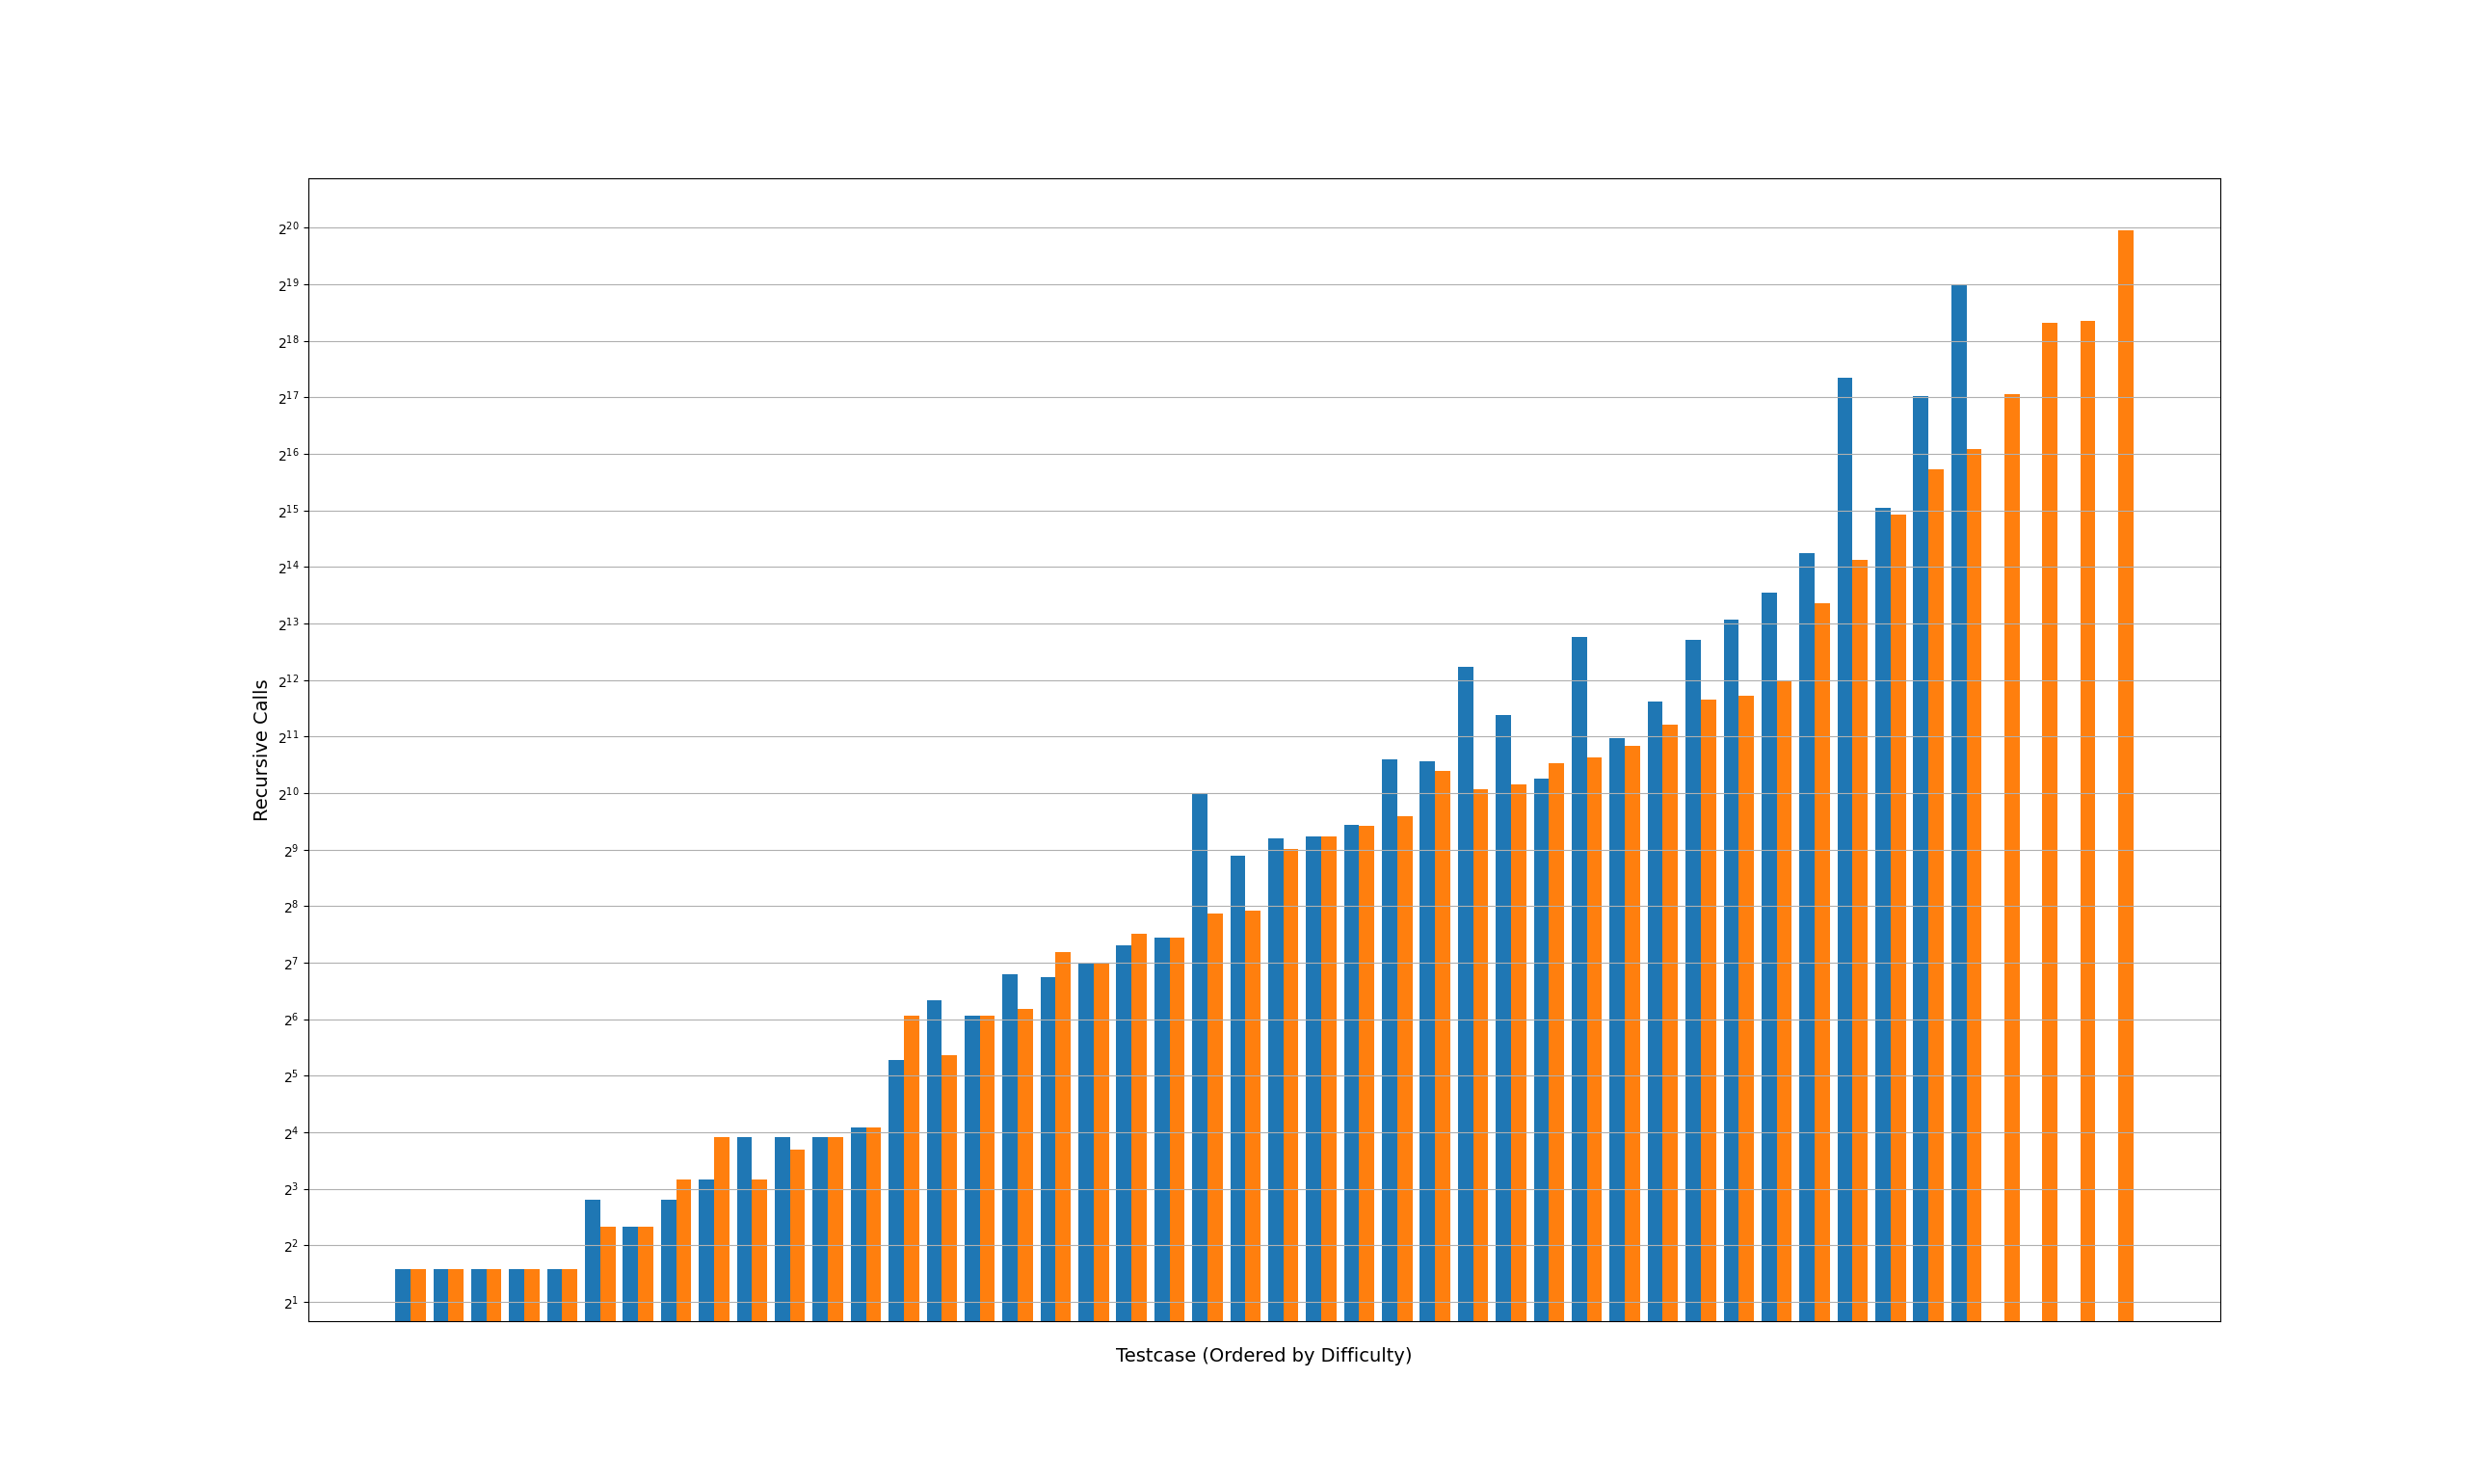
\includegraphics[scale=.5]{vertexedge.png} \end{center}

\newpage
\begin{center} Edge Rule vs. All Rules\\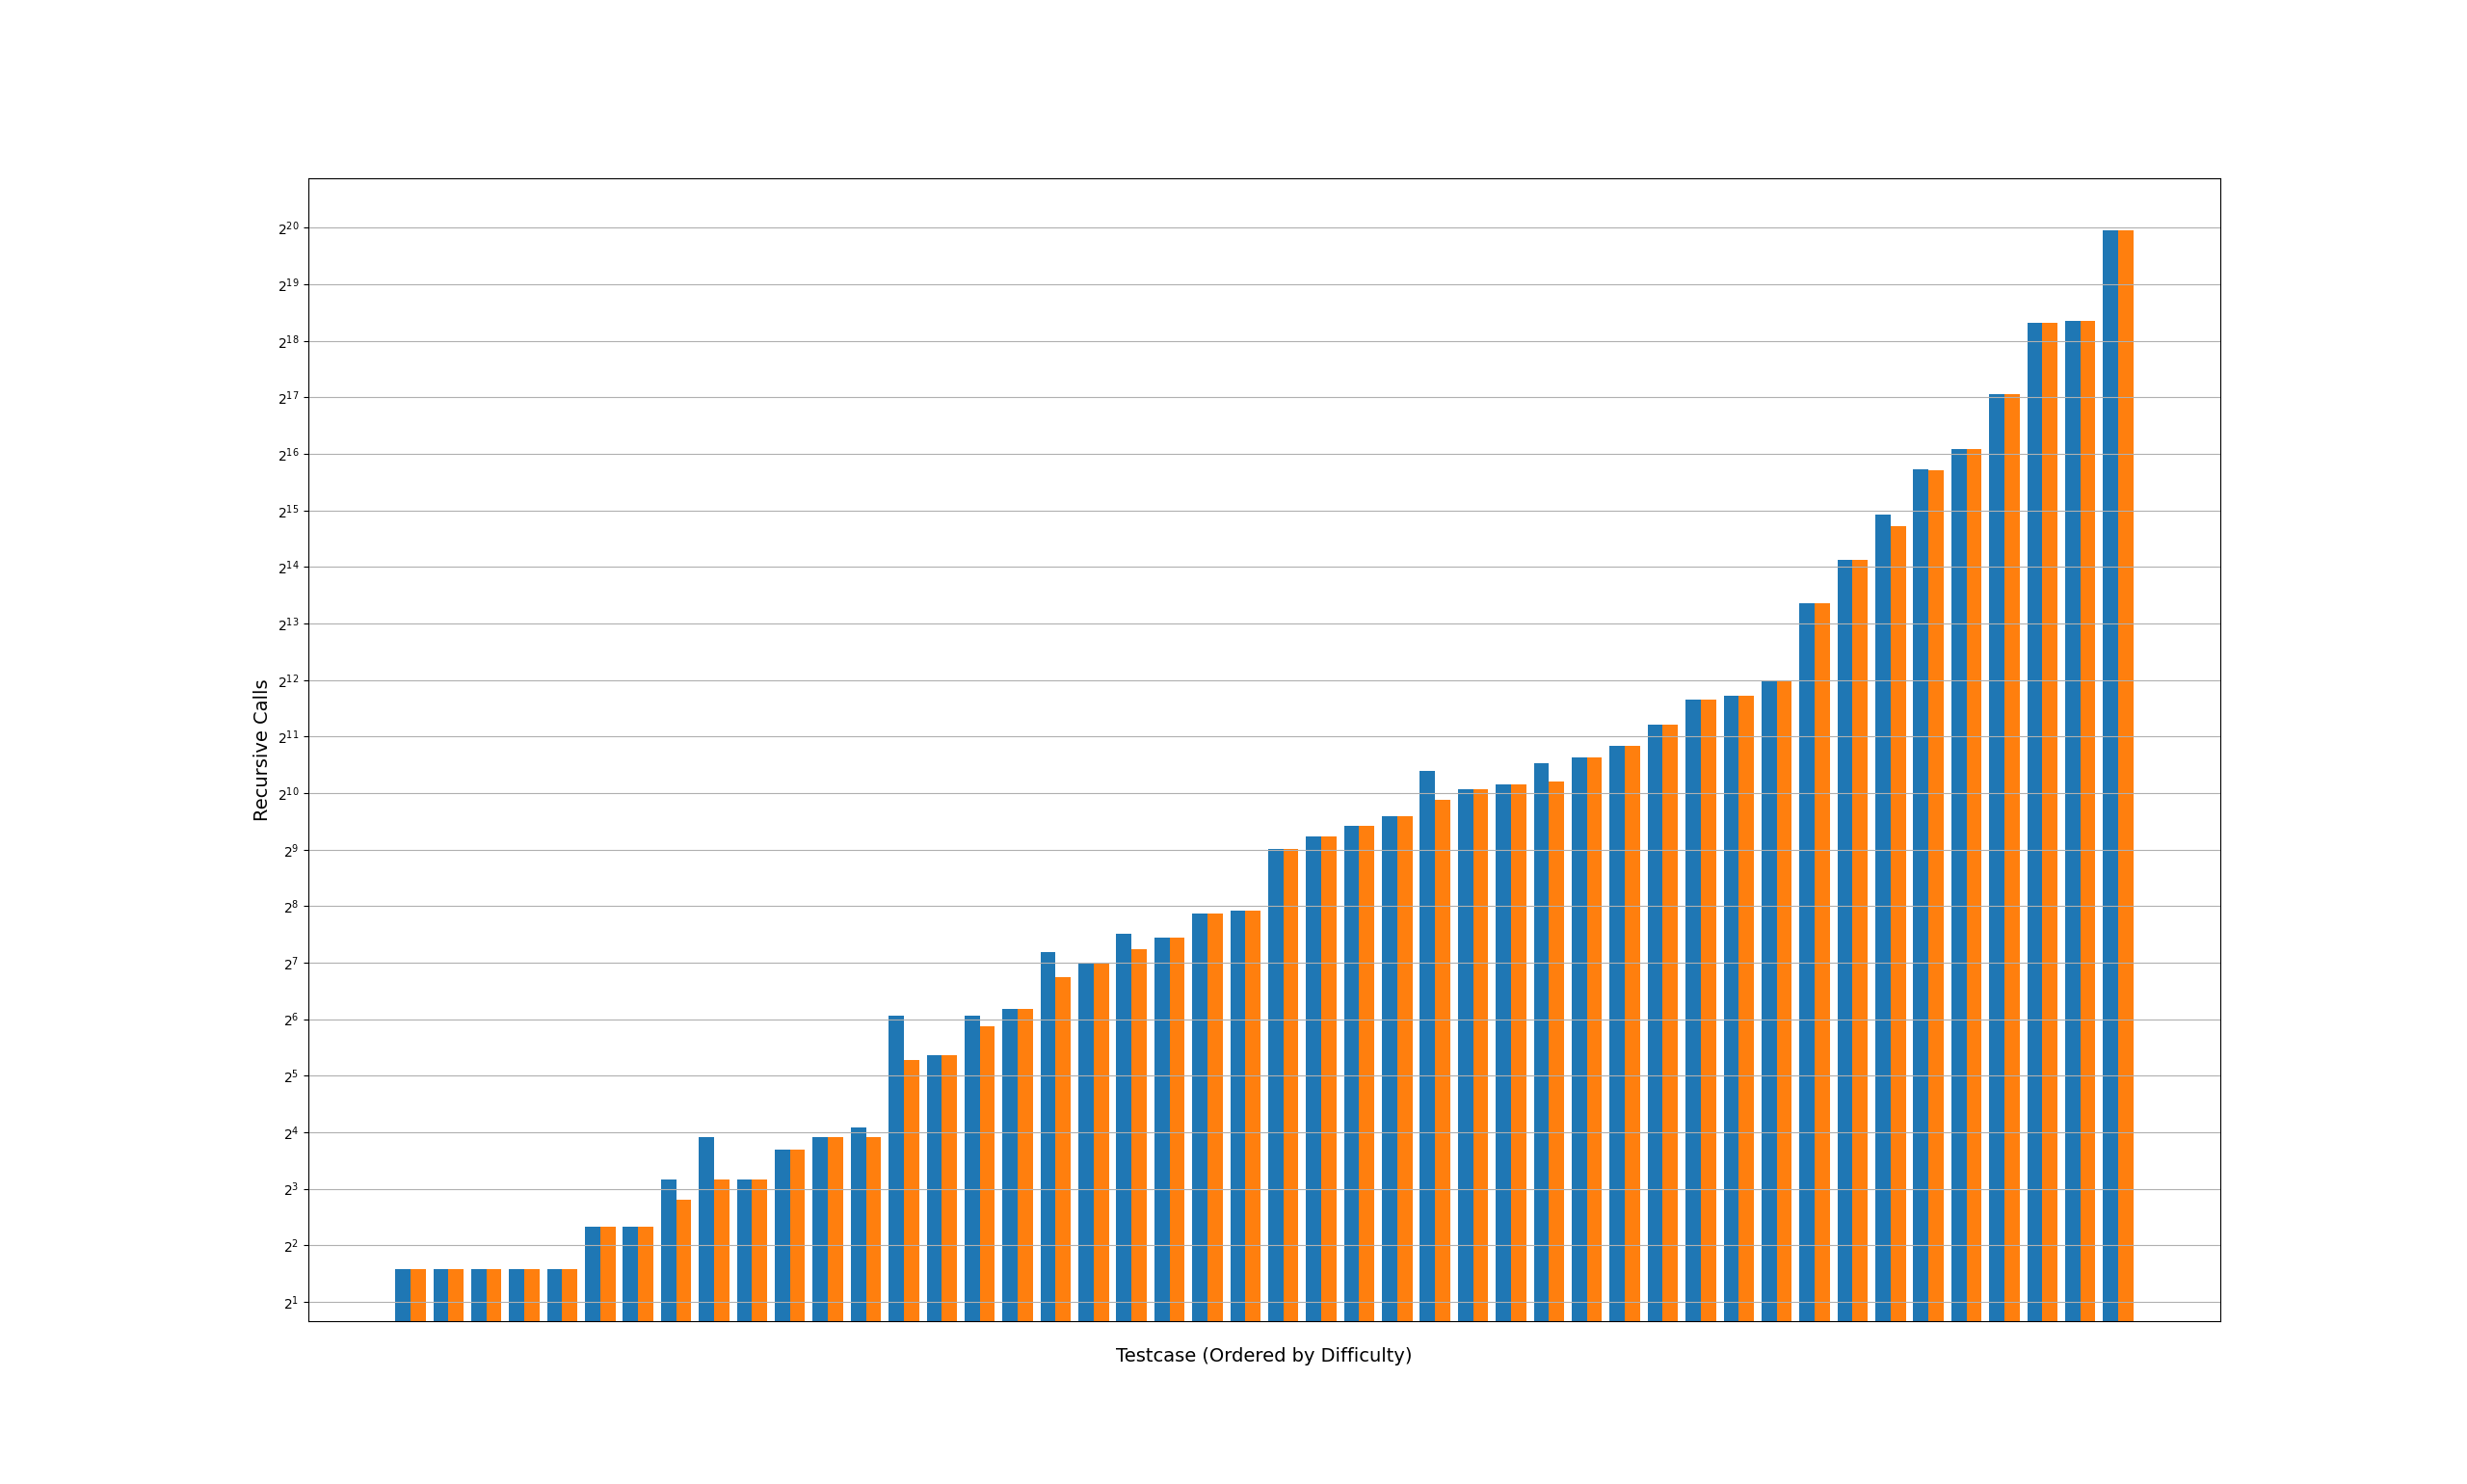
\includegraphics[scale=.5]{edgefull.png} \end{center}

\newpage
\begin{center} No Pruning vs. All Rules\\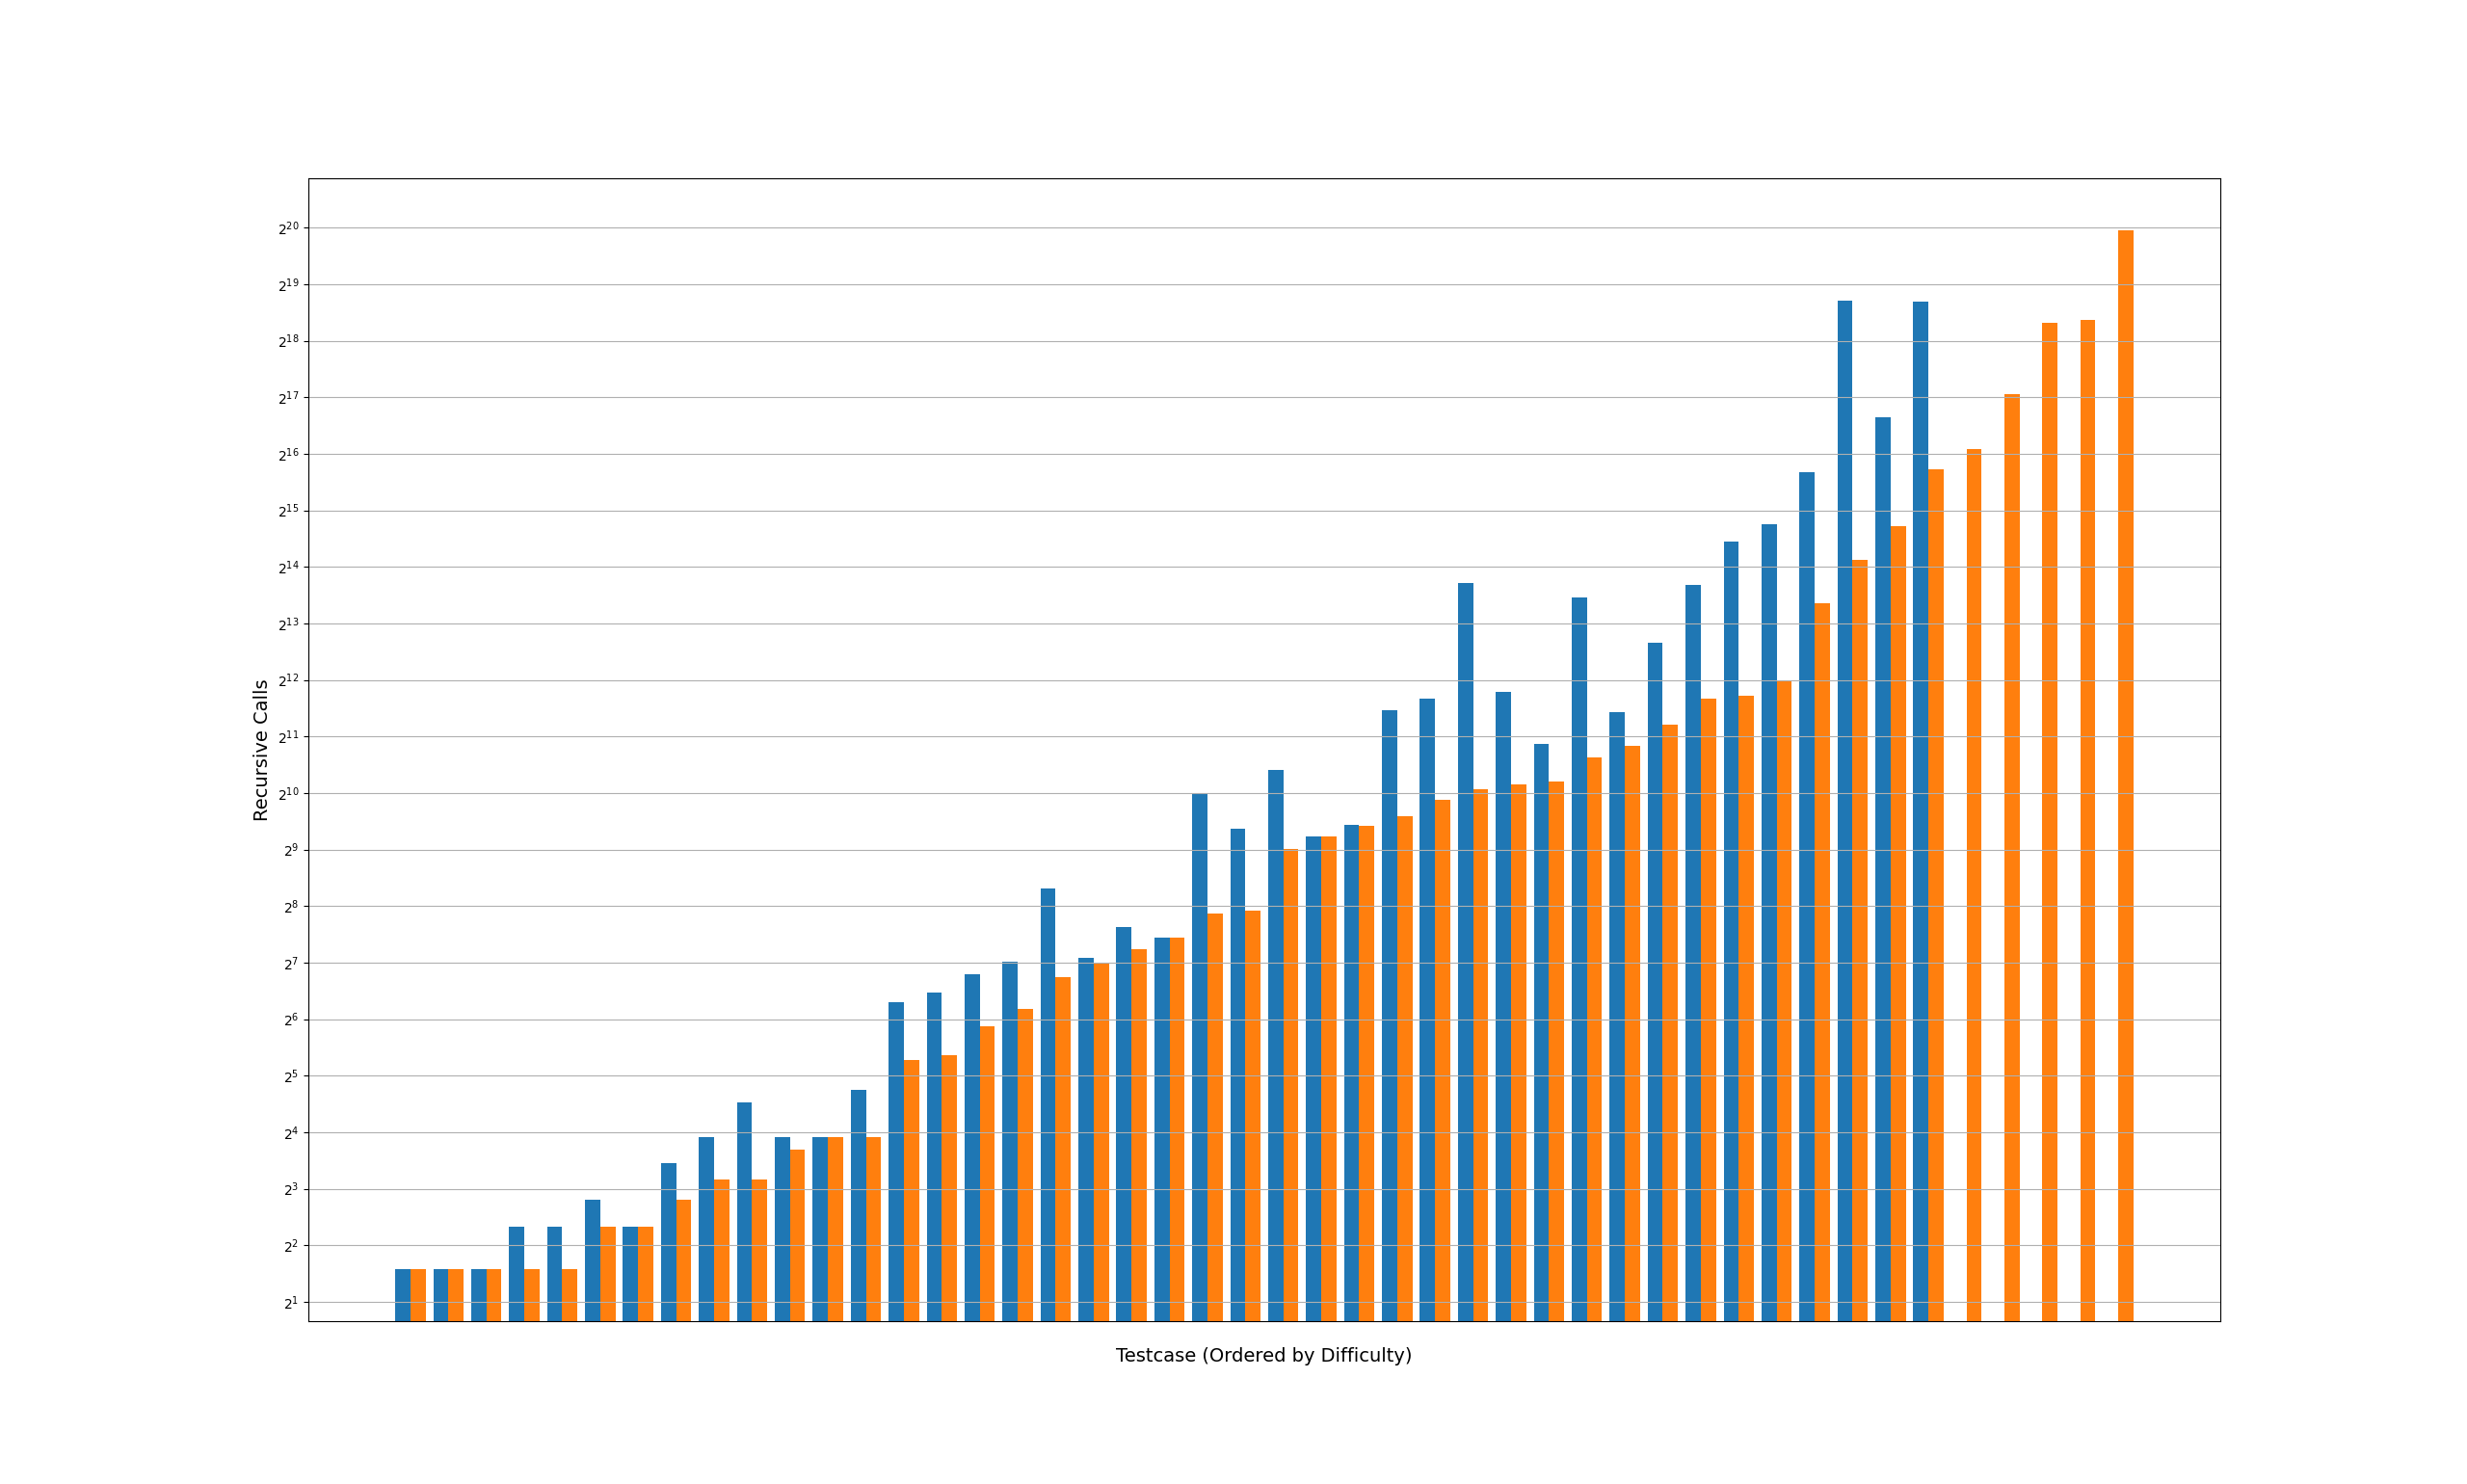
\includegraphics[scale=.5]{nonefull.png} \end{center}

\newpage
\begin{center} Random Edge Branching vs. Lowest Score Edge Branching\\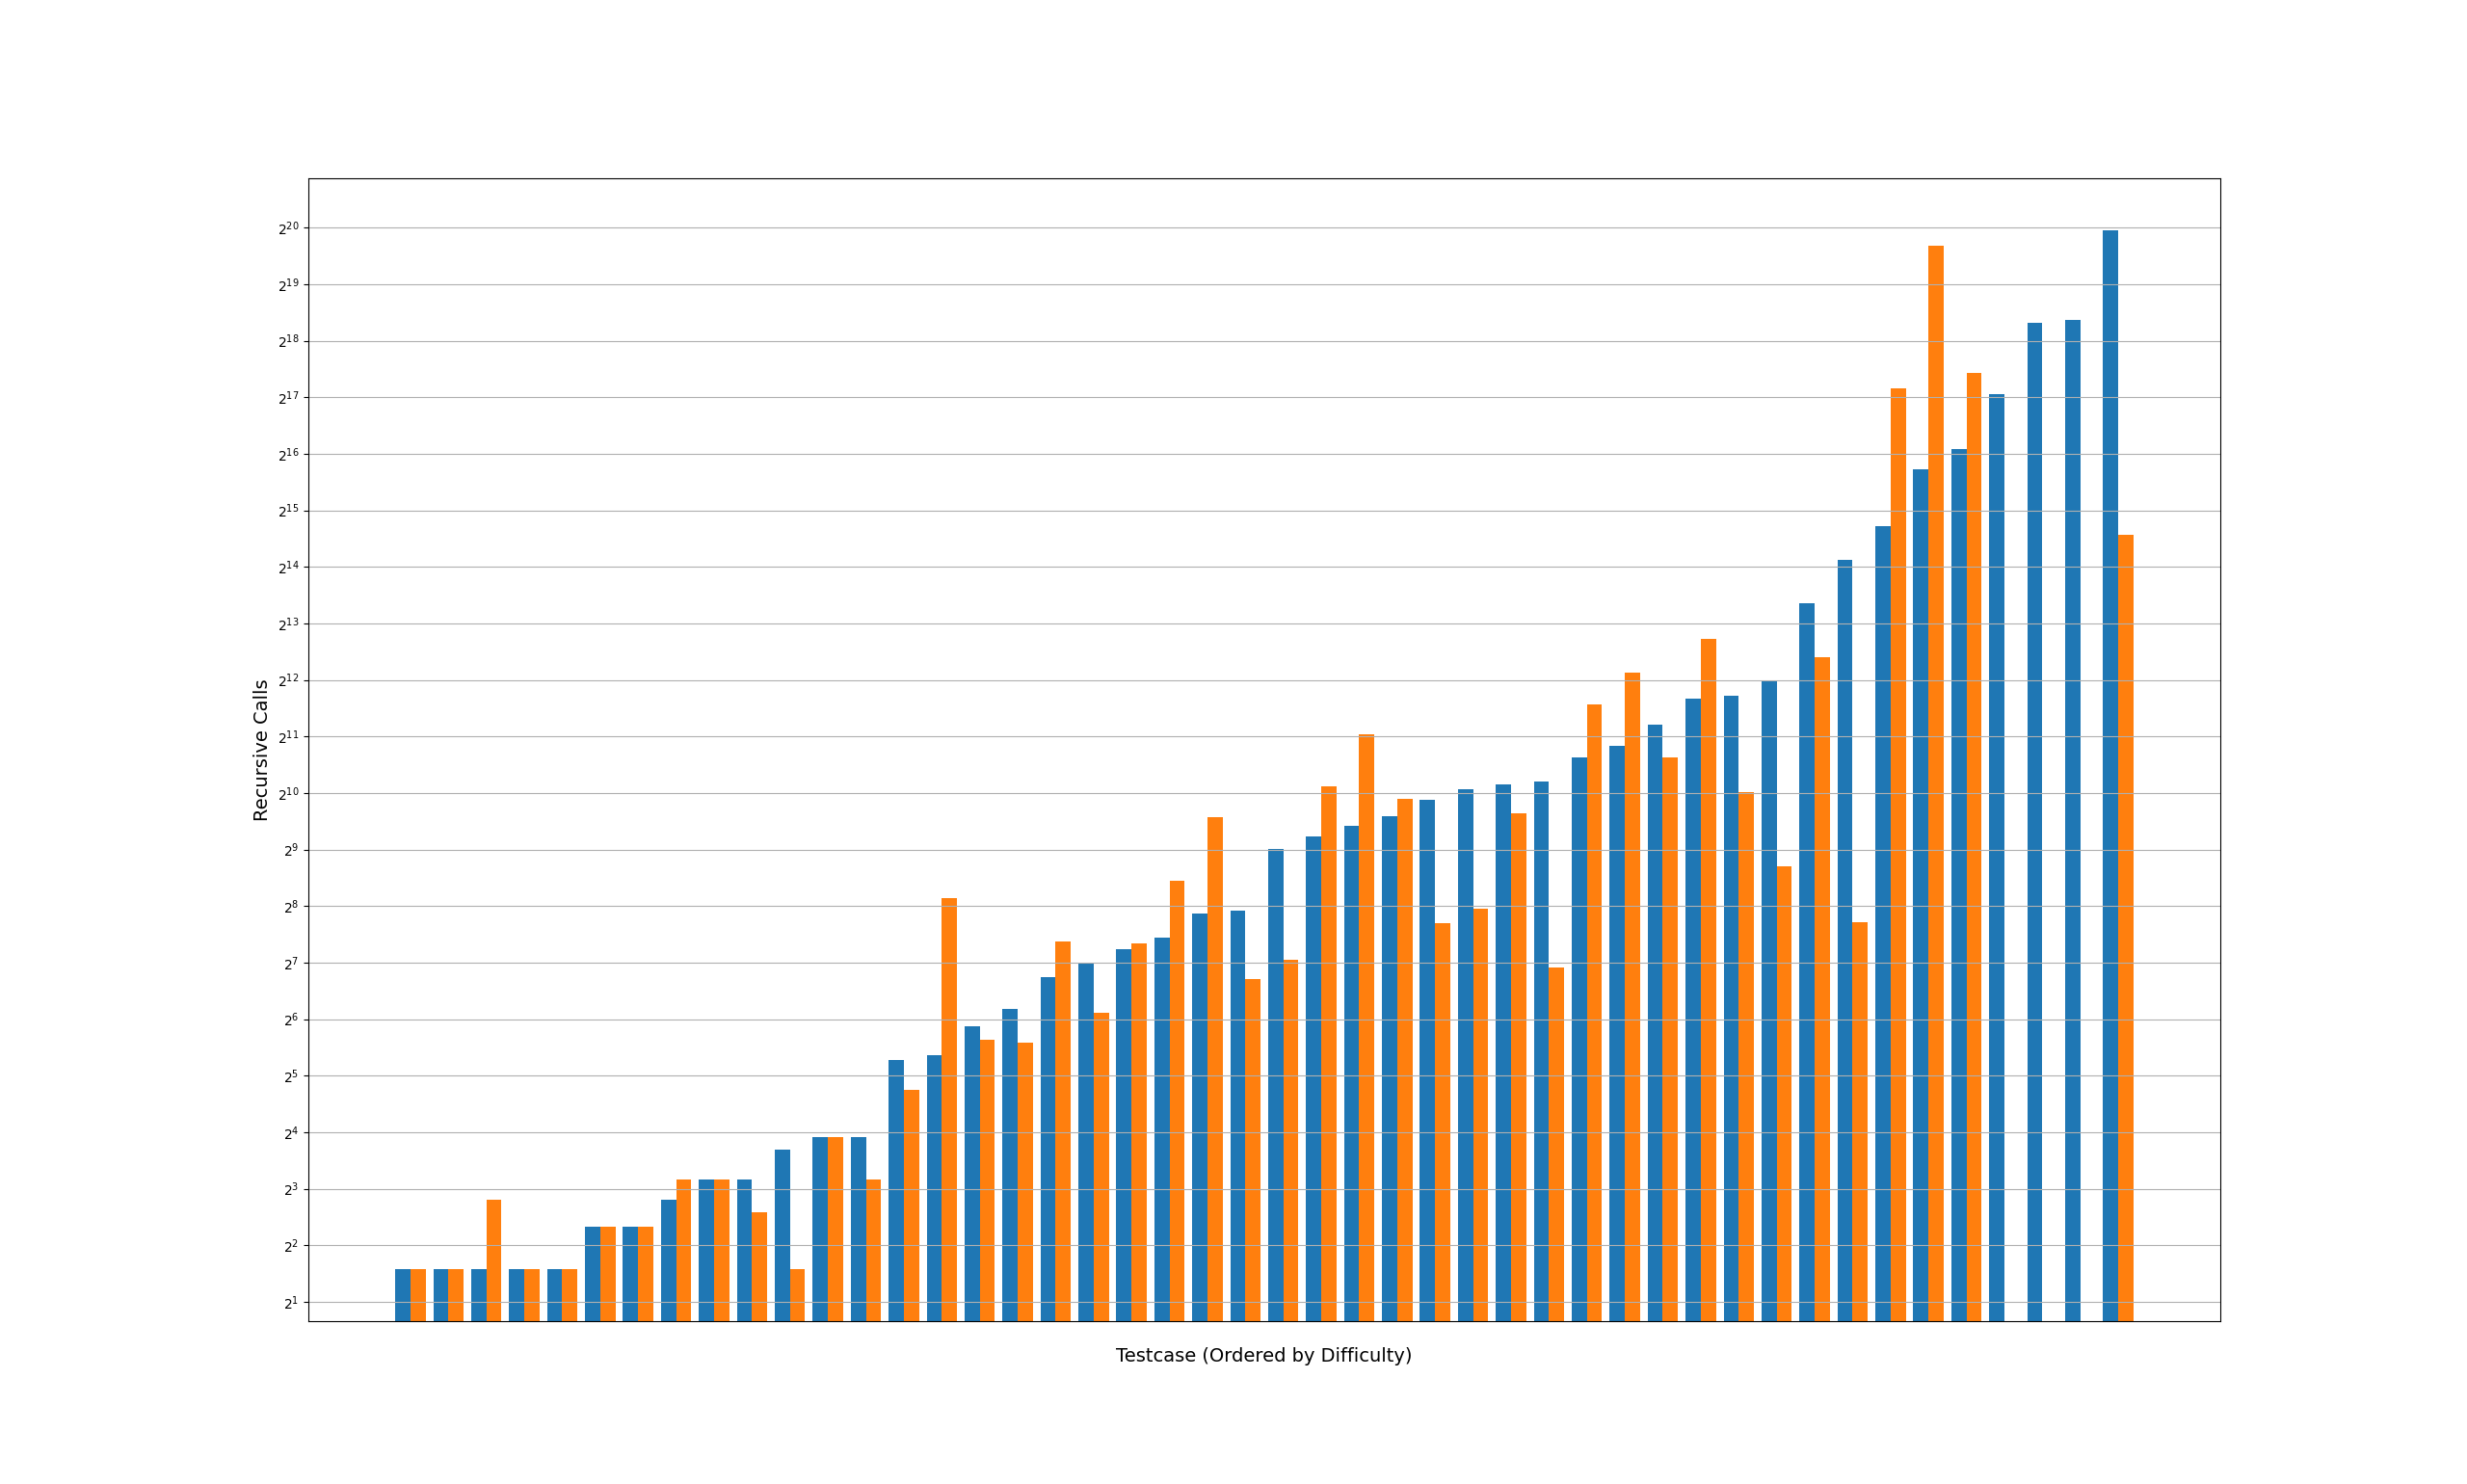
\includegraphics[scale=.5]{branching.png} \end{center}

\newpage
\section*{Thank You!}

\end{document}
